\chapter{Overall Description}

\section{Product Perspective}

This section contains scenarios and further information on the shared phenomena, as well as a domain model consisting of a class diagram and state charts.

\subsection{Class diagram}

The class diagram presented in figure \ref{fig:class_diagram} provides a high-level overview of the system. Below are brief descriptions of the purpose of each class.

\begin{itemize}
    \item User classes:
    
    \begin{itemize}
        \item \textbf{User:} an abstraction of a registered user, being a base of all the other user classes.
        \item \textbf{Agronomist:} a class modeling an agronomist described in section \ref{subsec:agronomist}.
        \item \textbf{Farmer:} identifies a farmer described in section \ref{subsec:farmer}.
        \item \textbf{PolicyMaker:} a class modeling a policy maker whose description is to be found in section \ref{subsec:policy_maker}.
    \end{itemize}
    
    \item Enumerators:
    
    \begin{itemize}
        \item \textbf{VisitState:} describes the status of agronomist's visit to a farm.
        \item \textbf{Note:} contains possible notes given to a farmer for his performance by a policy maker.
        \item \textbf{WeatherType:} contains all weather condition types handled by the system.
    \end{itemize}
    
    Responses from external systems:
    
    \begin{itemize}
        \item \textbf{SensorSystemResponse:} models a response from the sensors available on a farm.
        \item \textbf{WaterIrrigationSystemResponse:} models a response from the water irrigation system on a farm.
        \item \textbf{WeatherSystemResponse:} models a response from the system providing meteorological forecasts.
    \end{itemize}
    
    \item Others:
    
    \begin{itemize}
        \item \textbf{Farm:} identifies a farm.
        \item \textbf{Production:} a class modelling production on a given farm. It represents the amount of each type of crops produced. 
        \item \textbf{ProductionType:} identifies a type of produced crops.
        \item \textbf{Mandal:} identifies a local government area in India.
        \item \textbf{Visit:} a class modelling agronomist's visit on a farm.
        \item \textbf{HelpRequest:} a class representing a farmer's request for help.
        \item \textbf{HelpResponse:} a class representing a response to a request for help.
        \item \textbf{ForumThread:} identifies a discussion forum created by a farmer.
        \item \textbf{ForumComment:} identifies comments posted on a discussion forum.
    \end{itemize}    
\end{itemize}

\begin{figure}[H]
    \centering
    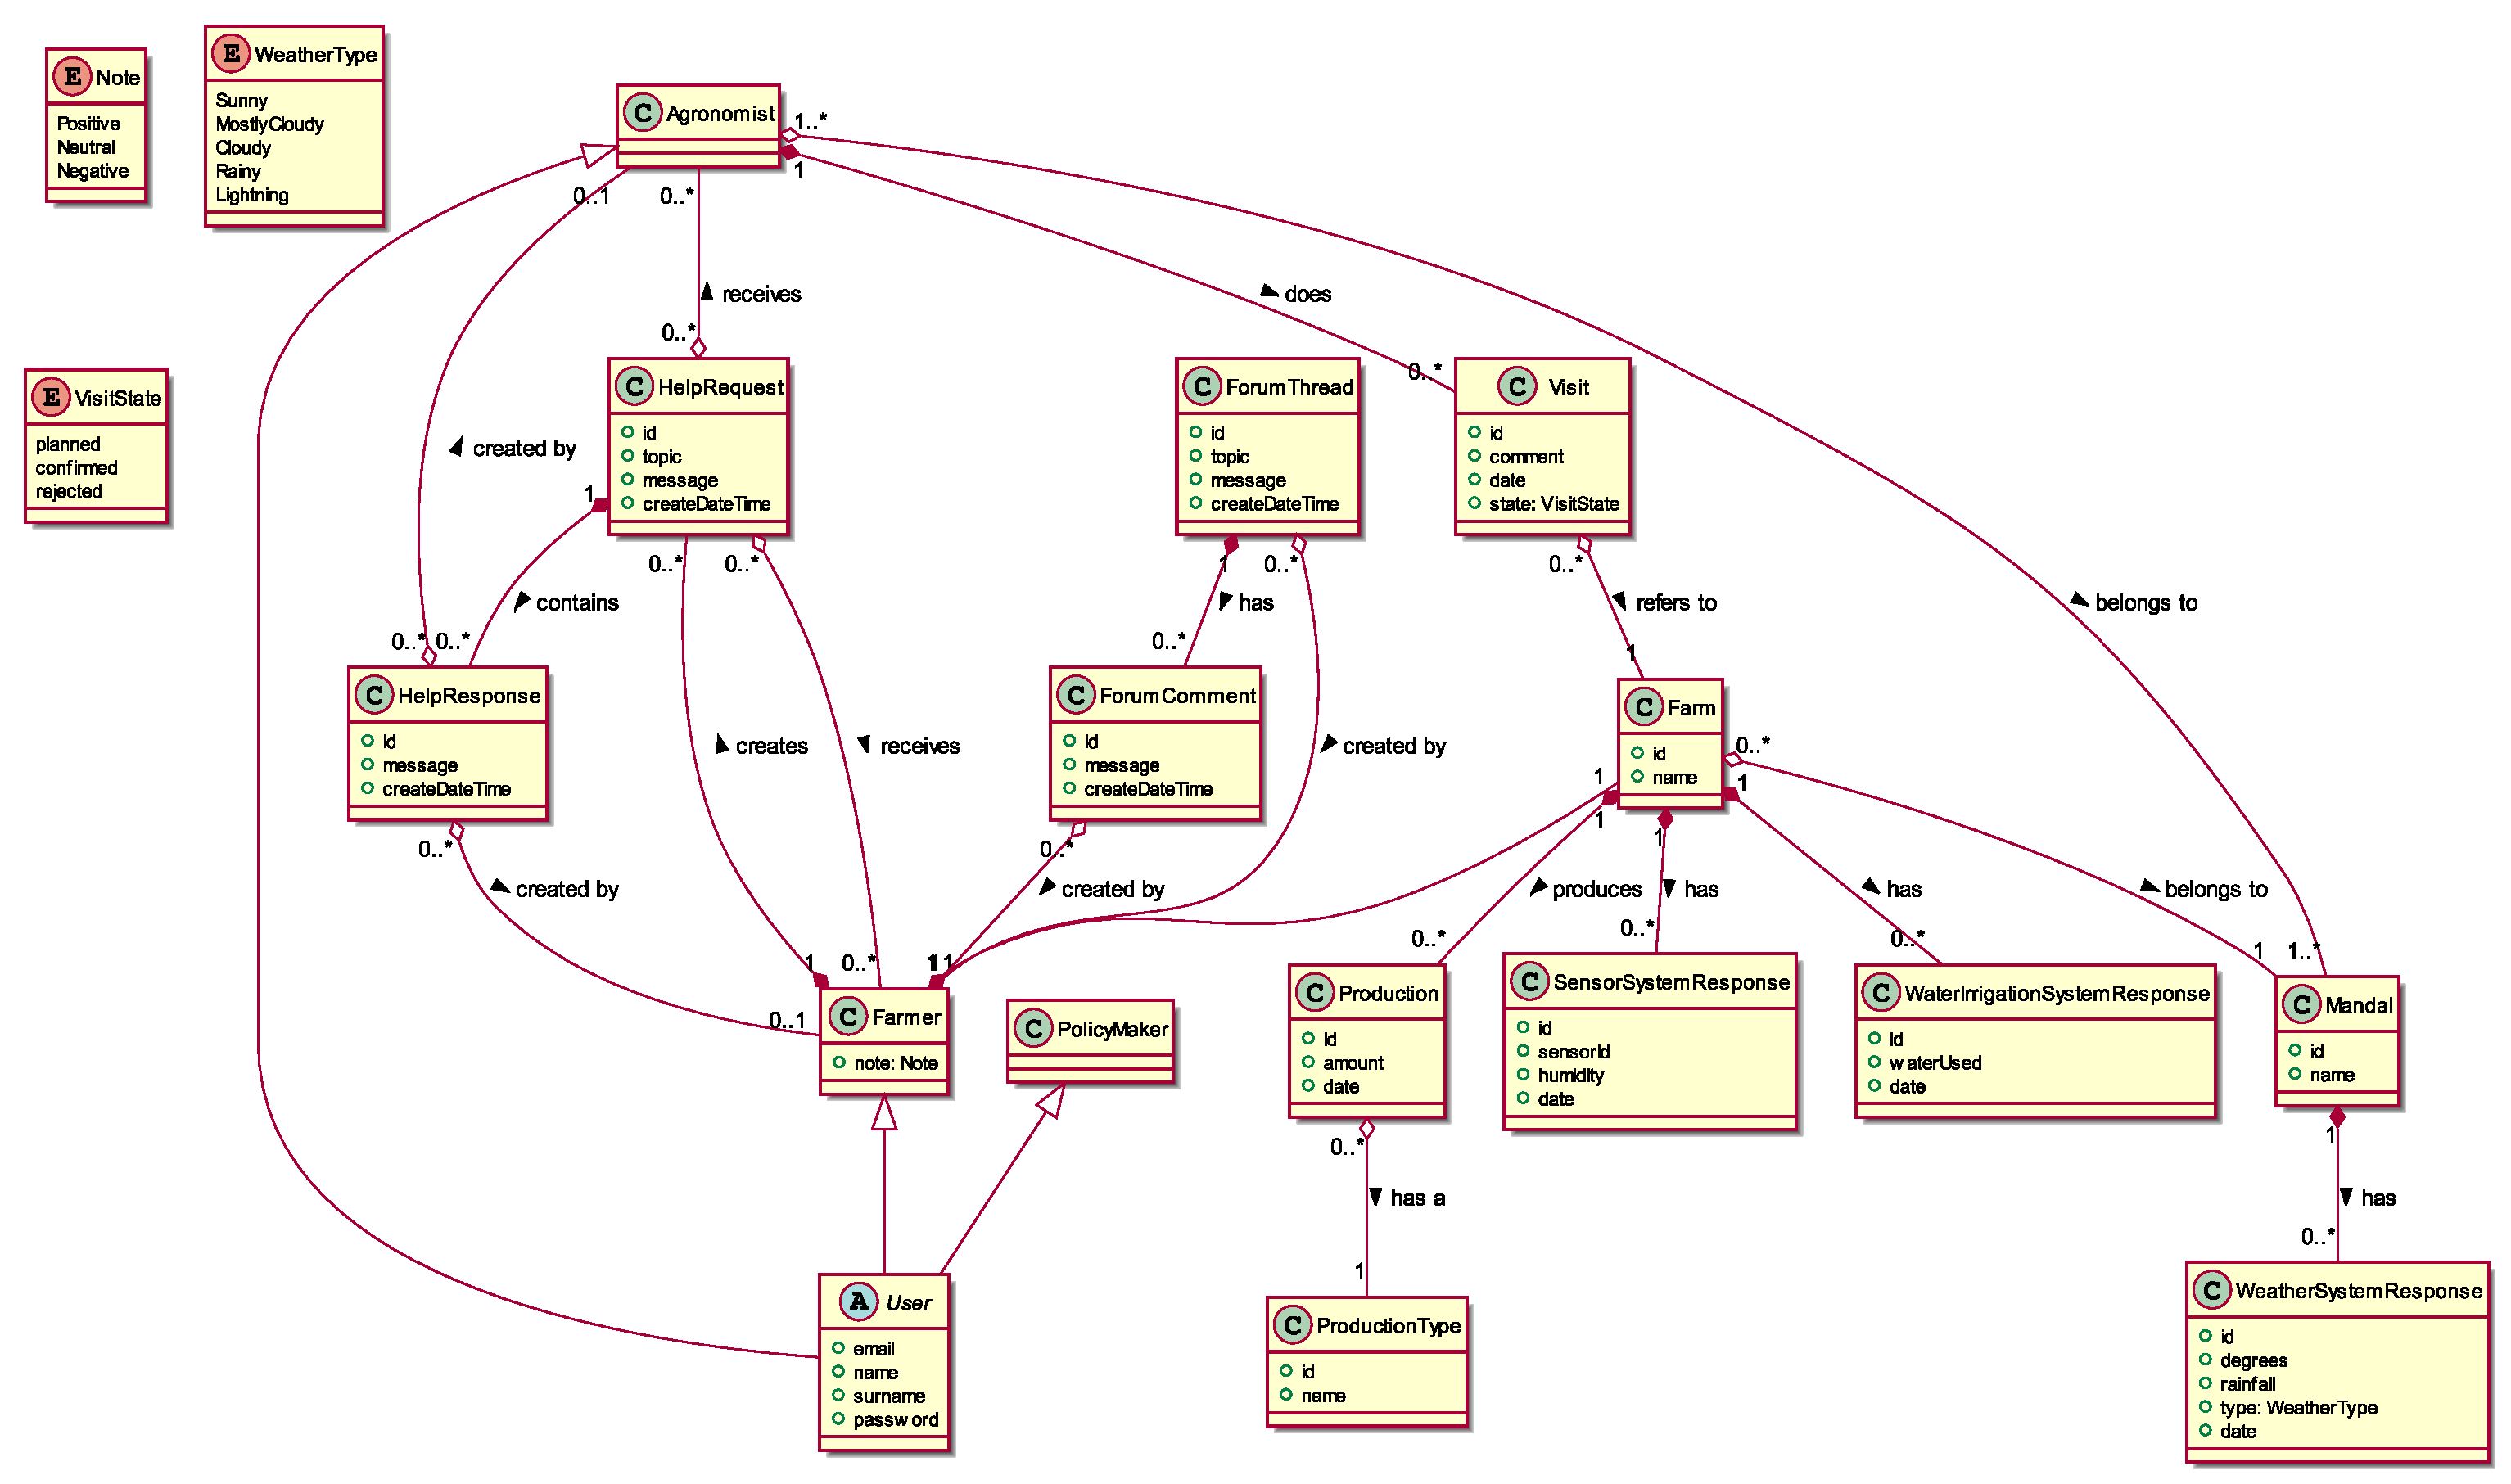
\includegraphics[width=0.96\textheight, keepaspectratio, origin=c, angle=90]{diagrams/class}
    \caption{Class diagram}
    \label{fig:class_diagram}
\end{figure}

\subsection{State diagrams}

The system was designed to be stateless except for the event of an agronomist visiting a farm. The event-ordered behavior of an object of the \textit{VisitState} class is presented in the figure \ref{fig:state_diagram}.

\begin{figure}[H]
    \centering
    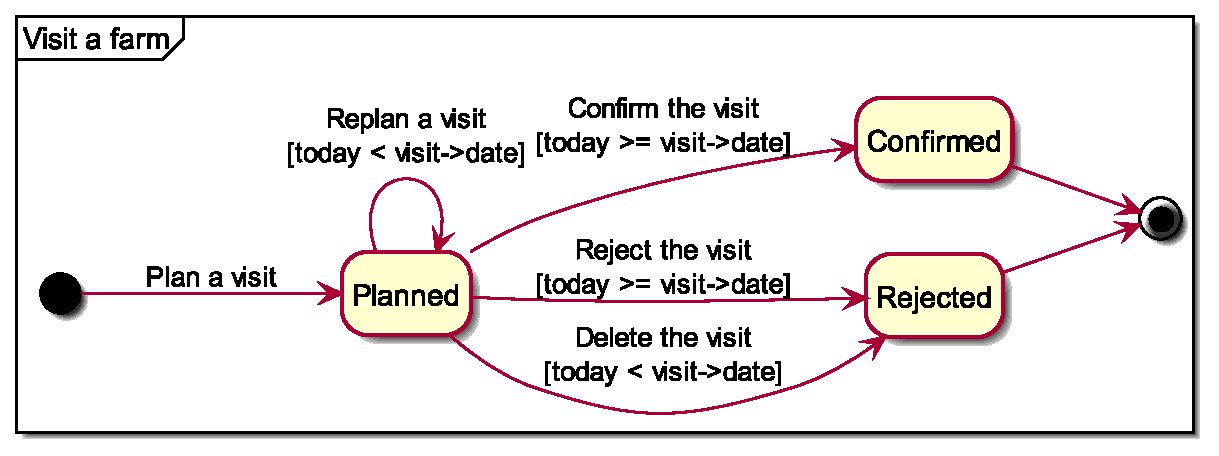
\includegraphics[width=\textwidth, keepaspectratio, origin=c]{diagrams/state}
    \caption{State diagram presenting an agronomist's visit on a farm}
    \label{fig:state_diagram}
\end{figure}

% scenarios
% use cases

\subsection{Scenarios}
\subsection*{Farmer's performance assessment by a policy maker}
John, a policy maker, logs in to the application to see how farmers are performing. He goes through the list of farmers and notices that despite very dry weather conditions in the region, the Joe Sharma's production of carrots has significantly increased. John gives Sharma's a positive note, and then he continues to look at the list of farmers. He spots that the production of Tamia Anand and Amar Khatri has plunged. He thinks it may be an effect of droughts that were reported in the system. He gives both farmers a negative note, hoping that other farmers and agronomists will be able to help them. 

\subsection*{An agronomist and a farmer help a farmer who obtained a negative note}
Dream automatically creates and delegates the requests for help about poorly performing farmers to both the agronomists in the given area of responsibility and farmers with positive notes. As a result, an agronomist, Rajesh Khanna, receives requests that indicate the farmers with negative note. Rajesh looks through the farmers' summaries, to determine any possible reasons for the farmers' bad performance. In the case of Tamia Anand's, he notices that her irrigation system entries from the last month show understated values. Rajesh uses a response option to advise Tamia to check if the system is working properly. 

The same requests are also obtained by a farmer, Trisha Gupta, who  recently obtained a positive note. She shares some general advices about dealing with adverse weather conditions in the mandal using the response option.

\subsection*{Policy maker checks whether a farmer obtained proper help}
Shaila, a policy maker, is already logged in to the application. She wants to see if farmers with negative notes are obtaining proper help. Therefore, she looks at the farmer's summary belonging to Amar Khatri, who was marked with a negative note. She reads the advice provided by both agronomists working in the area and Joe Sharma, who is a farmer with a positive note. Joe Sharma shared some best practices on how to deal with droughts in the farm. Shaila wants to wait to see if the production of Amar Khatri will improve in the following month, but is happy to see that the farmer obtained meaningful advices.

\subsection*{A farmer reads individualized recommendations}
Ishaan Patel grows potatoes and wants to prepare a planting plan of his farm. For that reason, he opens the application and looks for a weather forecast in his region. Ishaan finds out that it is going to rain next weekend, but afterwards the weather will be perfect for planting. Hence, he decides to start planting next Monday. Next to the weather forecasts, among farmer's relevant data, Ishaan reads a recommendation about potassium salt that can be used to increase the potato crops. As a result, Ishaan thinks about including potassium salt fertilization in his planting plan. 

\subsection*{A farmer inserts production data}
Shalene Reddy assessed that she produced 40 tons of rice on her farm in the last month. She logs in to the application and updates the production data. She looks through the history of her production entries to verify whether she is on the right track. 

\subsection*{A farmer requests for help}
Nalin Laghari experiences difficulties on his cotton farm. He is striving to fight off bollworms. Thus, he wants to create a request for help in the application. He opens the application and describes the details of his problems with bollworms.

The application automatically delegates a request for help to both the agronomists in the given area of responsibility and well-performing farmers nearby. As a result, an agronomist, Devraj Jain receives a request for help. Devraj knows some theory as well as several practices that farmers used before to deal with bollworms, so he shares some hints in a response to the request. The same request is also obtained by a farmer, Joe Sharma. Joe recommends one of the insecticides in the response, since he successfully fought off bollworms a year ago.

\subsection*{A farmer creates a discussion forum}
Paidi Jairaj has a large carrot farm in Jagtial. Lately, he heard some rumors about potato farming becoming more and more profitable. He is wondering if it is worth switching his type of production to another type of crops in the next season. He wants to reach other farmers in his mandal to get to know their opinion. To do this, Paidi logs into DREAM application and chooses the option to create a discussion thread, in which he specifies the topic and description of his dilemma.

Gajam Anjaiah, a potato farmer from Jagtial, logs in to DREAM application to check, if there are any interesting discussions on the discussion forum. He sees Paidi's thread, and knowing a lot about potatoes production, creates a comment in the thread, containing various advice and remarks concerning potato's production.

\subsection*{An agronomist manages daily plan}
Zakir Hussain, a governmental agronomist, wants to visualize and check his daily plan. He logs in to DREAM app, chooses the option to see plan and then clicks on the following day. After reading the generated plan, he realizes that he will be driving near Syed Nayeemuddin's farm, who recently asked for help. He decides to alter his plan to visit Syed's farm. He chooses the option to edit the plan, types Syed's name in a search bar and chooses him from the list, which contains suggestions of farmers in Zakir's area of responsibility, as well as information regarding how many times they were visited in the current year. Lastly, Zakir confirms the edits he made.

\subsection*{An agronomist sets daily plan's execution state}
Zakir Hussain, a governmental agronomist, has finished today's farm visits. During visits, he collected some comments about conditions of the farms. Unfortunately, he couldn't visit one of the farms. Zakir logs into DREAM app, chooses the option to see daily plan, and then clicks on the current day. In the daily plan view, he clicks ona button to set the daily plan's execution state. A pop-up appears, which tells him to specify deviations from the plan, indicating which farms he has and hasn't visited. For every farm he has visited, Zakir fills a short note. After completing the form, he confirms daily plan's execution.

The application automatically plans new visits to farms that were visited. In case a farm was not visited, the application plans another approximately 5 days later.

\subsection*{An agronomist responds to a farmer’s request for help} 
Sachindranath Mitra, a governmental agronomist, wants to check if any farmer in his area of responsibility needs help. He logs into DREAM app and sees a new help request in the dashboard from Paidi Jairaj. He chooses the option to manage help requests and clicks on Paidi's request. A pop-up appears, which allows him to provide advice. After filling the form, the response is sent to the farmer.

\subsection*{An agronomist looks at the list of well performing farmers}
Jarnail Singh, a governmental agronomist, wants to check if there is any new well-performing farmer in his area of responsibility. He logs into DREAM app, and on the dashboard he sees a quick summary, containing the weather forecast for the day and some best performing farmers. He clicks on the option to see full summary, which allows him to see a complete list of all the well-performing farmers in the area of responsibility. 

\section{Product Functions}

This section provides a summary of the major functions that the system will introduce to achieve the goals outlined in the section \ref{subsec:goals}.

\subsection{Registration}
% Area of responsibility for agronomists, crops for farmers. Farm creation
The system allows for registration of three different types of users: agronomists, farmers, and policy makers. Characteristics of each user are described in the section \ref{sec:user_characteristics}.

\subsubsection*{Agronomist}

\begin{itemize}
    \item Provides email and password.
    \item Inserts his area of responsibility.
\end{itemize}

\subsubsection*{Farmer}

\begin{itemize}
    \item Enters email and password.
    \item Introduces relevant data regarding the location of his farm.
\end{itemize}

\subsubsection*{Policy maker}

\begin{itemize}
    \item Inserts email and password.
\end{itemize}

Additionally, the system introduces a functionality to reset a forgotten password. The user needs to press on a dedicated button and provide his email address. He will later receive a link to a webpage where he will be able to introduce a new password. 

\subsection{Performance assessment of the farmers}
% Water irigation systems, sensors.

DREAM system utilizes external services such as water irrigation systems and sensors measuring the humidity of the soil to extract valuable data. Based on that, together with production data which is updated by a farmer, and the weather conditions, a policy maker is able to assess the performance of a farmer by assigning him a positive, negative, or neutral note.

\subsection{Update production data (farmer)}

The system allows a farmer to update his production data. It is required to specify the type of crops as well as their quantity produced during the entire month. This data is further used for the performance assessment of each farmer.

\subsection{Request for help}
% together with a response

Using DREAM enables farmers to request assistance and advice from agronomists and other farmers in a convenient way. The system asks them to create an issue by describing their problems, and subsequently sends  requests to all the agronomists and well-performing farmers from the same mandal. Then each of the recipients can provide help. The track of the issue remains visible only to the people involved as well as the policy makers.

\subsection{Coordinate agronomist's daily plan}

Each farm should be inspected at least twice a year, but those that are underperforming should be visited more frequently, depending on the nature of the problem. The system automates these visits by developing a daily plan for each agronomist, which is accessible via the dashboard. Furthermore, at the end of each day, an agronomist can validate the completion of the daily plan or identify deviations from it.

\subsection{Create discussion forum}

The system provides also a possibility for a farmer to freely create discussion forums with other farmers. Such threads do not have any restrictions on their topic. They can include suggestions, queries, and even off-topic material. Each farmer can participate in a certain thread by leaving a comment. All forum threads are visible to all the registered farmers.

\subsection{Visualize farmer's relevant data}

The system enables farmers to display data relevant to them, such as weather forecasts and tailored recommendations for certain crops to plant or fertilizers to utilize, based on their region and kind of production. This information will be visible on the main dashboard after logging in to the system.

\section{User Characteristics} \label{sec:user_characteristics}

DREAM is a project whose key component is data acquisition and integration. All of this is used to support the work of three distinct types of registered actors: agronomists, farmers, and policy makers. Additionally, there is a description of an unregistered user provided.

\subsection{Agronomist} \label{subsec:agronomist}

% Who he is
In the realm of agriculture, an agronomist serves as an intermediary between farmers and policy makers. He advises farmers on soil management and crop production.

% What he does
Governmental agronomists in the Telangana region visit farms in their areas of responsibility on a frequent basis to acquire information regarding farmers' performance.

% How the system helps him in achieving his goal
The system provides many functionalities in order to make agronomists' job more convenient. Firstly, it allows an agronomist to insert his area of responsibility. Then, it provides them with visualizations depicting best performing farmers in the region as well as weather forecasts. To help manage their schedule, it creates an interactive daily plan to visit farms for them, where they can confirm its execution and also specify any deviations from it. Additionally, the system significantly facilitates their contact with the farmers by notifying them about incoming help requests and providing an easy way to respond to them directly.

\subsection{Farmer} \label{subsec:farmer}

% Who he is
This actor is directly involved in Telangana's food production. He owns a farm where he raises crops that are later distributed around the region.

% What he does
During the production process, a farmer faces many difficulties caused by external factors such as weather conditions.

% How the system helps him in achieving his goal
To assist a farmer in accomplishing his objective, the system allows him to set up his own profile where he can share his production data. Moreover, it provides information important to him, such as tailored advice about which crops to plant or which fertilizers to use depending on his location and kind of production, as well as weather forecasts. Furthermore, it enables him to create discussion forums, where he could share his difficulties and solicit recommendations or assistance from agronomists and other farmers.

\subsection{Policy maker} \label{subsec:policy_maker}

% Who he is
A member of Telangana's governmental department, which is in charge of developing new rules and legislation pertaining to food production.

% What he does
His primary responsibility is to ensure that new policies help to increase food production by monitoring farmers' productivity data.

% How the system helps him in achieving his goal
The system's purpose is to help them identify which farmers are performing well and which are not. With this kind of help, a policymaker can more correctly assign notes to farmer's performance and understand if the steering initiatives carried out by agronomists with the support of excellent farmers create major outcomes thanks to the data obtained by the system.

\subsection{Unregistered user}

An individual belonging to one of the aforementioned groups who is not yet registered in the system.

\section{Assumptions, Dependencies and Constraints}

\subsection{Assumptions}

\begin{longtable}{@{}p{0.06\linewidth} p{0.88\linewidth}}
		\toprule
		\textbf{ID}   & \textbf{Assumption}\\
		\midrule
     \autonum{A} & Each farmer possess exactly one farm.\\
     \autonum{A} & Each farm belongs to exactly one farmer.\\ 
     \autonum{A} & Each farm has at least one humidity sensor.\\ 
     \autonum{A} & Each farm has an irrigation system.\\ 
     \autonum{A} & Each farm is inside exactly one mandal.\\ 
     \autonum{A} & Each farmer reliably updates his production data each month.\\ 
     \autonum{A} & Weather is consistent in a given mandal.\\ 
     \autonum{A} & Initially, each farmer has a neutral note.\\ 
     \autonum{A} & Agronomist's area of responsibility contains at least one mandal.\\ 
     \autonum{A} & Each registered user can be only one of the actors: an agronomist, a farmer, or a policy maker.\\ 
     \autonum{A} & The information provided by a user during registration process is valid.\\ 
     \autonum{A} & Well-performing farmers and agronomists are eager to help farmers with negative notes.\\ 
     \autonum{A} & Each mandal has at least one agronomist who is responsible for the farms inside that area.\\ 
     \autonum{A} & Based on farmer's summary, a policy maker is able to understand whether the help given by farmers and agronomists produces significant results.\\ 
     \autonum{A} & Farmers create meaningful and not offensive threads and comments on the forum.\\ 
     \autonum{A} & Farmers and agronomists create meaningful and not offensive help requests and responses. \\
     \autonum{A} & NEW \todo{verify new assumptions}\\
     \autonum{A} & External systems are reliable and highly available.\\
     \autonum{A} & Every sensor system has a unique ID assigned by sensor system provider. \\
     \autonum{A} & Every water irrigation system has a unique ID assigned by water irrigation system provider. \\
	\bottomrule
\end{longtable}
